\documentclass[mathserif, aspectratio=169]{beamer}

% Set up root path as macro
\makeatletter
\def\@rootpath{/Users/hainguyenvan/Desktop/presentations/2025_SIAM_CSE_Presentation/Latex/}
\newcommand{\fromroot}[1]{\@rootpath#1}
\def\input@path{{\@rootpath}}

% Define graphics path using the root path macro
\usepackage{graphicx}
\makeatletter
\newcommand{\setgraphicspath}{%
    \graphicspath{{\@rootpath}}%
}
\makeatother

% Call the macro to set graphics path
\setgraphicspath

% Input template using fromroot command
\input{\fromroot{template/template_1.tex}}

\begin{document}

% Input slides using fromroot command
\input{\fromroot{slides/slide_title.tex}}
\input{\fromroot{slides/slide_inverse_and_forward_problems.tex}}
\input{\fromroot{slides/slide_challenges.tex}}
\input{\fromroot{slides/slide_surrogates.tex}}
\frame{
\frametitle{Problem settings}
\vspace{-6ex}
% \bluebox{Problem settings}
{\small
We consider 
\begin{itemize}
    \item The linear forward problem
    \begin{equation*}
        \yb = B \circ \underbrace{G \ub}_{\omb} + \delta,
    \end{equation*}
    where $B$ is observational operator, $G$ is linear forward map, and $\delta$ is white noise. 
    
    \item The equivalent linear inverse problem
    \begin{equation*}
        \ub = \LRp{B \circ G}^\dagger \yb = {\GB}^\dagger \yb.
    \end{equation*}
\end{itemize}

We want to learn linear autoencoder surrogate models 
\begin{itemize}
    \item Encoder $\Psie(\yb) = \W_e \yb + \bb_e$ for inverse map ${\GB}^\dagger$.
    \item Decoder $\Psid(\ub) = \W_d \ub + \bb_d$ for forward map $G$ or PtO map $G^B$.
\end{itemize}

}

}}
\frame{
\frametitle{Autoencoder (AE) approaches}
\bluebox{We discuss}
{
    \begin{enumerate}
        \item Naive Autoencoder ($\pureOPO$)
        \item Model-constrained Autoencoder ($\mcOPO$)
        \item Tikhonov Autoencoder Network Approach ($\TNetAE$)
    \end{enumerate}
}
}





}
\frame{
\frametitle{Naive Autoencoder ($\pureOPO$) - error estimation}
\vspace{-3ex}
{\small
Given a dataset of pairs $\LRc{\P, \Y}$, we can learn forward and inverse surrogate models by 
\begin{equation*}
    \begin{aligned}
        & \text{first optimizing the encoder} & \Psie^* = & \min_{\Psie} \halfv{1} \nor{\Psie\LRp{\Y} - \P}_{F}^2, \\ 
        & \text{then decoder with pre-trained encoder}  & \Psid^* = & \min_{\Psid}  \halfv{1} \nor{\Psid\LRp{\Psie^*\LRp{\Y}} - \Y}_{F}^2.
    \end{aligned}
\end{equation*}

Applying 1st optimality condition for the optimal solutions $\Psie^*$ and $\Psid^*$, we have  
\begin{itemize}
    \item \myred{test inverse solution error}
    \[
        \epsb_{\ubtest}^{\pureOPO} = \nor{\Psie^*(\ybtest) - \ubtest }_2^2 = \nor{ \LRp{\bar{\P} \bar{\Y}^\dagger \GB -\Ib} \LRp{\ubtest - \bar{\ub}}}_2^2.
    \]
    \item \myred{test forward solution error}, with $Z = \Psie^*(\Y)$ is the encoder inverse solution, 
    \[
    \epsb_{\ybtest}^{\pureOPO} = \nor{\Psid^*(\ubtest) - \ybtest }_2^2  = \nor{\bar{\Y} \myblue{\LRp{\bar{Z}^{\dagger} - \bar{\P}^\dagger}} \LRp{\ubtest - \bar{\ub}}}_2^2 \myblue{> 0}, \]
    % where $\bar{\ub} = \frac{\P \One}{n_t}$ is the average of PoI samples, and $\bar{\P} = \P - \bar{\ub}\One^T$ is the centralized data, \\
    % \quad \quad \quad $Z = \Psie^*(\Y)$ is the encoder inverse solution.
\end{itemize}
}
}





}
\input{\fromroot{slides/slide_mc_AE_scheme_phase_1.tex}}
\input{\fromroot{slides/slide_mc_AE_scheme_phase_1_cont.tex}}
\input{\fromroot{slides/slide_mc_AE_scheme_phase_2.tex}}
\input{\fromroot{slides/slide_mc_AE_scheme_phase_2_cont.tex}}
\frame{
    \frametitle{Model-constrained Autoencoder ($\mcOPO$) - error estimation}
{\small
$\mcOPO$ loss functions
\begin{equation*}
    \begin{aligned}
\Psie^* = \min_{\Psie} & \halfv{1} \nor{\U - \Psie\LRp{\Y}}_{F}^2 + \halfv{\lambda}\nor{\Y - \GB\LRp{\Psie\LRp{\Y}}}_{F}^2, \\ 
        \Psid^* = \min_{\Psid} & \halfv{1} \nor{\G\LRp{\Psie^*\LRp{\Y}} -\Psid\LRp{\Psie^*\LRp{\Y}}}_{F}^2.
    \end{aligned}
\end{equation*}
Applying 1st optimality condition, and \myblue{\bf if $\bar{Y}$ is a full row rank}, we have  
\begin{itemize}
    \item \myred{test inverse solution error}
    \[
        \epsb_{\ubtest}^{\mcOPO} = \nor{\textcolor{red}{\left(\Ib + \lambda {\GB}^T{\GB}\right)^{-1}} \LRp{  \LRp{\bar{\P} \bar{\Y}^{\dagger} \GB - \Ib } \LRp{\ub^\text{test} - \bar{\ub}} } }_2^2 
    \]
    which is smaller than
    \[
        \epsb_{\ubtest}^{\pureOPO} = \nor{ \LRp{\bar{\P} \bar{\Y}^\dagger \GB -\Ib} \LRp{\ubtest - \bar{\ub}}}_2^2.
    \]
    \item \myred{test forward solution error}
    \[
    \epsb_{\ybfulltest}^{\mcOPO} = 0.
    \]
\end{itemize}
}
}}
\frame{
\frametitle{Key issue of $\mcOPO$: Error estimation is data-dependent}
Recall the test inverse solution error
\[
    \epsb_{\ubtest}^{\mcOPO} = \nor{\left(\Ib + \lambda {\GB}^T{\GB}\right)^{-1} \LRp{  \LRp{\textcolor{red}{\bar{\P} \bar{\Y}}^{\dagger} \GB - \Ib } \LRp{\ub^\text{test} - \textcolor{red}{\bar{\ub}}} } }_2^2 
\]
where 
\begin{itemize}
    \item $\textcolor{red}{\bar{\P}, \bar{\Y}}$ is centralized training data.
    \item $\textcolor{red}{\bar{\ub}}$ is the average of training PoI samples.
\end{itemize}

\vspace{2ex}

\myred{If training data $\P, \Y$ is limited, surrogate models heavily bias on given training data. \newline
Hence, leading to high test inverse error.}

\vspace{2ex}

\myblue{Our TAEN approach is introduced to deal with this issue}
}

}
\frame{
\frametitle{TAEN: Tikhonov Autoencoder Network Approach}
{\small
Recall the $\mcOPO$ loss functions
\begin{equation*}
    \begin{aligned}
        \Psie^* = \min_{\Psie} & \halfv{1} \nor{{\mygreen\U} - \Psie\LRp{\Y}}_{F}^2 + \halfv{\lambda}\nor{\Y - \GB\LRp{\Psie\LRp{\Y}}}_{F}^2, \\ 
        \Psid^* = \min_{\Psid} & \halfv{1} \nor{\G\LRp{\Psie^*\LRp{\Y}} -\Psid\LRp{\Psie^*\LRp{\Y}}}_{F}^2.
    \end{aligned}
\end{equation*}
In TAEN, we use the prior mean of PoI, $\mygreen{\ub_0}$, thus true PoI samples are no longer required.
\begin{equation*}
    \begin{aligned}
\Psie^* = \min_{\Psie} & \halfv{1} \nor{\mygreen{\ub_0 \One^T} - \Psie\LRp{\Y}}_{F}^2 + \halfv{\lambda}\nor{\Y - \B \circ \G\LRp{\Psie\LRp{\Y}}}_{F}^2, \\ 
        \Psid^* = \min_{\Psid} & \halfv{1} \nor{\G\LRp{\Psie^*\LRp{\Y}} -\Psid\LRp{\Psie^*\LRp{\Y}}}_{F}^2.
    \end{aligned}
\end{equation*}
Applying 1st optimality condition, and \myblue{\bf if $\bar{Y}$ is a full row rank}, we have 
\begin{itemize}
    \item \myred{test inverse solution error}
        \[
            \epsb_{\ubtest}^{\mcOPO} \leq  \nor{{\ub^\text{test} - {\ub}_0} }_2^2
        \]
    \item \myred{test forward solution error}
        \[
        \epsb_{\ybfulltest}^{\mcOPO} = 0, 
        \]
\end{itemize}
}
}}
\input{\fromroot{slides/slide_mc_AE_Y_full_row_rank.tex}}
\frame{
\frametitle{Summary of error estimation}
\bluebox{Error estimation on test samples}
{
    % \begin{table}[htb!]
    %     \centering
    %     \resizebox{1.\textwidth}{!}{
    %     \begin{tblr}{
    %       width = 1.2\linewidth,
    %       colspec = {X[c,m,1] X[c,m,1.4] X[c,m,2.2] X[c,m,1.4]},
    %       cell{2}{3} = {r=2}{},
    %       cell{4}{3} = {r=2}{},
    %       vlines,
    %       hline{1-2,4,6-7} = {-}{},
    %       hline{3,5} = {1-2,4}{},
    %     }
    %     Approaches    & {PtO/forward error \\ $\epsb_{\ybtest}$/ $\epsb_{\ybfulltest}$} & {Inverse error \\  $\epsb_{\ubtest}$}                                                           & {Ability to learn \\ with 1 sample} \\
    %     {\purePOP} & 0                         & $\nor{ \LRp{\bar{\P} \bar{\Y}^\dagger \GB -\Ib} \LRp{\ubtest - \bar{\ub}}}_2^2$   & None                            \\
    %     {\pureOPO} & inevitably \textgreater{} 0           &                                                                                   & None                            \\
    %     {\mcPOP}        & 0                         & $\le \nor{ \LRp{\bar{\P} \bar{\Y}^\dagger \GB -\Ib} \LRp{\ubtest - \bar{\ub}}}_2^2$ & Only PtO                            \\
    %     {\mcOPO}        & 0                         &                                                                                   & Only forward                            \\
    %     {\myred{\texttt{TAEN}}}        & 0                         & $\le \nor{{\ub^\text{test} - \ub_0}}_2^2$                                            & \myred{All}                           
    %     \end{tblr}
    %     }
    % \end{table}

    \begin{table}[htb!]
        \centering
       \resizebox{1.\textwidth}{!}{
       \begin{tblr}{
        width = 1.2\linewidth,
        colspec = {X[c,m,1] X[c,m,1.4] X[c,m,2.2] X[c,m,1.4]},
        vlines,
        hline{1-2,3-5} = {-}{},
        }
        Approaches & {forward error \\ $\epsb_{\ybtest}$/ $\epsb_{\ybfulltest}$} & {Inverse error \\ $\epsb_{\ubtest}$} & {Ability to learn \\ with 1 sample $\yb$} \\
        {\pureOPO} & inevitably \textgreater{} 0 & $\nor{ \LRp{\bar{\P} \bar{\Y}^\dagger \GB -\Ib} \LRp{\ubtest - \bar{\ub}}}_2^2$ & none \\
        {\mcOPO} & 0 & $\le \nor{ \LRp{\bar{\P} \bar{\Y}^\dagger \GB -\Ib} \LRp{\ubtest - \bar{\ub}}}_2^2$ & only forward \\
        {\myred{\texttt{TAEN}}} & 0 & $\le \nor{{\ub^\text{test} - \ub_0}}_2^2$ & {forward and inverse} \\
       \end{tblr}
        }
       \end{table}

    
}
\begin{itemize}
    % \item With only one observation sample $\yb$, {\myred{\texttt{TAEN}}} can 
    % \begin{itemize}
    %     \item[-] learn exactly the forward map
    %     \item[-] provide the best inverse solution error estimation.
    % \end{itemize}
    \item Please see our preprint for discussions for non-linear problems.
\end{itemize}

}}
\input{\fromroot{slides/slide_numerical_results_overal.tex}}
\frame{
\frametitle{2D Heat equation}

\vspace{-4ex}
{
    \begin{align*}
    -\nabla \cdot \LRp{e^u \nabla \omega}    & = 20  \quad \text{in } \Omega = \LRp{0,1}^2 \\
    \omega                                   & = 0 \quad \text{ on } \Gamma^{\text{ext}}   \\
    \textbf{n} \cdot \LRp{e^u \nabla \omega} & = 0 \quad \text{ on } \Gamma^{\text{root}},
\end{align*}
}

% \begin{center}
%         \begin{figure}[htb!]
%             \begin{center}
%                 \resizebox{.8\textwidth}{!}{
%                 \begin{tabular*}{\textwidth}{c@{\hskip -0.01cm} c@{\hskip -0.01cm} c@{\hskip -0.01cm} }
%                     \centering
%                     Discretization & Conductivity & Temperature  \\
%                     \raisebox{-0.5\height}{\resizebox{0.33\textwidth}{!}{

% This file was created with tikzplotlib v0.10.1.
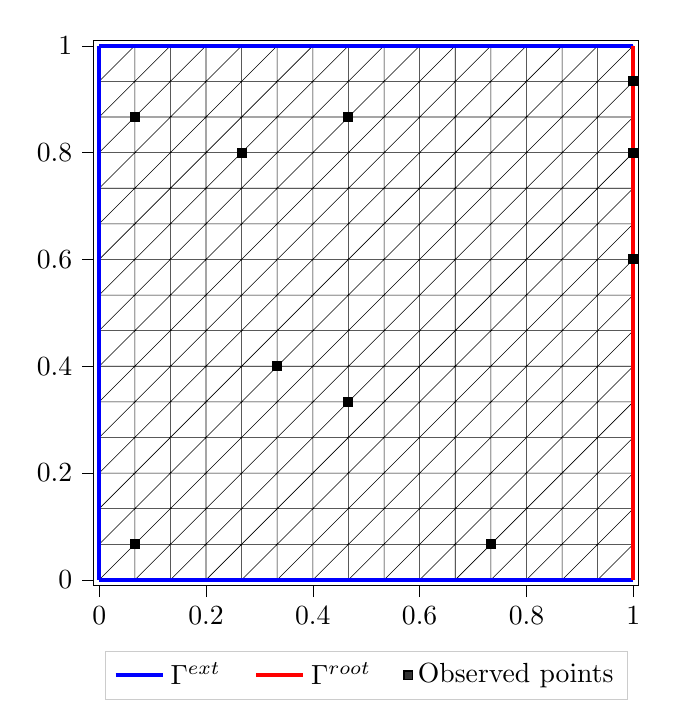
\begin{tikzpicture}

  \definecolor{darkgray176}{RGB}{176,176,176}
  \definecolor{lightgray204}{RGB}{204,204,204}
  
  \begin{axis}[
  % Set the aspect ratio to 1 for a square plot
  unit vector ratio*=1 1 1,
  % Set equal width and height
  width=8.5cm,
  height=8.5cm,
  legend cell align={left},
  legend columns=3,
  legend style={
    fill opacity=0.8,
    draw opacity=1,
    text opacity=1,
    at={(0.5,-0.12)},
    anchor=north,
    draw=lightgray204
  },
  tick align=outside,
  tick pos=left,
  unbounded coords=jump,
  x grid style={darkgray176},
  xmin=-0.01, xmax=1.01,
  xtick style={color=black},
  y grid style={darkgray176},
  ymin=-0.01, ymax=1.01,
  ytick style={color=black}
  ]
  \addplot [very thin, black, forget plot]
  table {%
  0.0666666666666667 0
  0 0
  nan nan
  0.133333333333333 0
  0.0666666666666667 0
  nan nan
  0.2 0
  0.133333333333333 0
  nan nan
  0.266666666666667 0
  0.2 0
  nan nan
  0.333333333333333 0
  0.266666666666667 0
  nan nan
  0.4 0
  0.333333333333333 0
  nan nan
  0.466666666666667 0
  0.4 0
  nan nan
  0.533333333333333 0
  0.466666666666667 0
  nan nan
  0.6 0
  0.533333333333333 0
  nan nan
  0.666666666666667 0
  0.6 0
  nan nan
  0.733333333333333 0
  0.666666666666667 0
  nan nan
  0.8 0
  0.733333333333333 0
  nan nan
  0.866666666666667 0
  0.8 0
  nan nan
  0.933333333333333 0
  0.866666666666667 0
  nan nan
  1 0
  0.933333333333333 0
  nan nan
  0 0.0666666666666667
  0 0
  nan nan
  0.0666666666666667 0.0666666666666667
  0 0
  nan nan
  0.0666666666666667 0.0666666666666667
  0.0666666666666667 0
  nan nan
  0.0666666666666667 0.0666666666666667
  0 0.0666666666666667
  nan nan
  0.133333333333333 0.0666666666666667
  0.0666666666666667 0
  nan nan
  0.133333333333333 0.0666666666666667
  0.133333333333333 0
  nan nan
  0.133333333333333 0.0666666666666667
  0.0666666666666667 0.0666666666666667
  nan nan
  0.2 0.0666666666666667
  0.133333333333333 0
  nan nan
  0.2 0.0666666666666667
  0.2 0
  nan nan
  0.2 0.0666666666666667
  0.133333333333333 0.0666666666666667
  nan nan
  0.266666666666667 0.0666666666666667
  0.2 0
  nan nan
  0.266666666666667 0.0666666666666667
  0.266666666666667 0
  nan nan
  0.266666666666667 0.0666666666666667
  0.2 0.0666666666666667
  nan nan
  0.333333333333333 0.0666666666666667
  0.266666666666667 0
  nan nan
  0.333333333333333 0.0666666666666667
  0.333333333333333 0
  nan nan
  0.333333333333333 0.0666666666666667
  0.266666666666667 0.0666666666666667
  nan nan
  0.4 0.0666666666666667
  0.333333333333333 0
  nan nan
  0.4 0.0666666666666667
  0.4 0
  nan nan
  0.4 0.0666666666666667
  0.333333333333333 0.0666666666666667
  nan nan
  0.466666666666667 0.0666666666666667
  0.4 0
  nan nan
  0.466666666666667 0.0666666666666667
  0.466666666666667 0
  nan nan
  0.466666666666667 0.0666666666666667
  0.4 0.0666666666666667
  nan nan
  0.533333333333333 0.0666666666666667
  0.466666666666667 0
  nan nan
  0.533333333333333 0.0666666666666667
  0.533333333333333 0
  nan nan
  0.533333333333333 0.0666666666666667
  0.466666666666667 0.0666666666666667
  nan nan
  0.6 0.0666666666666667
  0.533333333333333 0
  nan nan
  0.6 0.0666666666666667
  0.6 0
  nan nan
  0.6 0.0666666666666667
  0.533333333333333 0.0666666666666667
  nan nan
  0.666666666666667 0.0666666666666667
  0.6 0
  nan nan
  0.666666666666667 0.0666666666666667
  0.666666666666667 0
  nan nan
  0.666666666666667 0.0666666666666667
  0.6 0.0666666666666667
  nan nan
  0.733333333333333 0.0666666666666667
  0.666666666666667 0
  nan nan
  0.733333333333333 0.0666666666666667
  0.733333333333333 0
  nan nan
  0.733333333333333 0.0666666666666667
  0.666666666666667 0.0666666666666667
  nan nan
  0.8 0.0666666666666667
  0.733333333333333 0
  nan nan
  0.8 0.0666666666666667
  0.8 0
  nan nan
  0.8 0.0666666666666667
  0.733333333333333 0.0666666666666667
  nan nan
  0.866666666666667 0.0666666666666667
  0.8 0
  nan nan
  0.866666666666667 0.0666666666666667
  0.866666666666667 0
  nan nan
  0.866666666666667 0.0666666666666667
  0.8 0.0666666666666667
  nan nan
  0.933333333333333 0.0666666666666667
  0.866666666666667 0
  nan nan
  0.933333333333333 0.0666666666666667
  0.933333333333333 0
  nan nan
  0.933333333333333 0.0666666666666667
  0.866666666666667 0.0666666666666667
  nan nan
  1 0.0666666666666667
  0.933333333333333 0
  nan nan
  1 0.0666666666666667
  1 0
  nan nan
  1 0.0666666666666667
  0.933333333333333 0.0666666666666667
  nan nan
  0 0.133333333333333
  0 0.0666666666666667
  nan nan
  0.0666666666666667 0.133333333333333
  0 0.0666666666666667
  nan nan
  0.0666666666666667 0.133333333333333
  0.0666666666666667 0.0666666666666667
  nan nan
  0.0666666666666667 0.133333333333333
  0 0.133333333333333
  nan nan
  0.133333333333333 0.133333333333333
  0.0666666666666667 0.0666666666666667
  nan nan
  0.133333333333333 0.133333333333333
  0.133333333333333 0.0666666666666667
  nan nan
  0.133333333333333 0.133333333333333
  0.0666666666666667 0.133333333333333
  nan nan
  0.2 0.133333333333333
  0.133333333333333 0.0666666666666667
  nan nan
  0.2 0.133333333333333
  0.2 0.0666666666666667
  nan nan
  0.2 0.133333333333333
  0.133333333333333 0.133333333333333
  nan nan
  0.266666666666667 0.133333333333333
  0.2 0.0666666666666667
  nan nan
  0.266666666666667 0.133333333333333
  0.266666666666667 0.0666666666666667
  nan nan
  0.266666666666667 0.133333333333333
  0.2 0.133333333333333
  nan nan
  0.333333333333333 0.133333333333333
  0.266666666666667 0.0666666666666667
  nan nan
  0.333333333333333 0.133333333333333
  0.333333333333333 0.0666666666666667
  nan nan
  0.333333333333333 0.133333333333333
  0.266666666666667 0.133333333333333
  nan nan
  0.4 0.133333333333333
  0.333333333333333 0.0666666666666667
  nan nan
  0.4 0.133333333333333
  0.4 0.0666666666666667
  nan nan
  0.4 0.133333333333333
  0.333333333333333 0.133333333333333
  nan nan
  0.466666666666667 0.133333333333333
  0.4 0.0666666666666667
  nan nan
  0.466666666666667 0.133333333333333
  0.466666666666667 0.0666666666666667
  nan nan
  0.466666666666667 0.133333333333333
  0.4 0.133333333333333
  nan nan
  0.533333333333333 0.133333333333333
  0.466666666666667 0.0666666666666667
  nan nan
  0.533333333333333 0.133333333333333
  0.533333333333333 0.0666666666666667
  nan nan
  0.533333333333333 0.133333333333333
  0.466666666666667 0.133333333333333
  nan nan
  0.6 0.133333333333333
  0.533333333333333 0.0666666666666667
  nan nan
  0.6 0.133333333333333
  0.6 0.0666666666666667
  nan nan
  0.6 0.133333333333333
  0.533333333333333 0.133333333333333
  nan nan
  0.666666666666667 0.133333333333333
  0.6 0.0666666666666667
  nan nan
  0.666666666666667 0.133333333333333
  0.666666666666667 0.0666666666666667
  nan nan
  0.666666666666667 0.133333333333333
  0.6 0.133333333333333
  nan nan
  0.733333333333333 0.133333333333333
  0.666666666666667 0.0666666666666667
  nan nan
  0.733333333333333 0.133333333333333
  0.733333333333333 0.0666666666666667
  nan nan
  0.733333333333333 0.133333333333333
  0.666666666666667 0.133333333333333
  nan nan
  0.8 0.133333333333333
  0.733333333333333 0.0666666666666667
  nan nan
  0.8 0.133333333333333
  0.8 0.0666666666666667
  nan nan
  0.8 0.133333333333333
  0.733333333333333 0.133333333333333
  nan nan
  0.866666666666667 0.133333333333333
  0.8 0.0666666666666667
  nan nan
  0.866666666666667 0.133333333333333
  0.866666666666667 0.0666666666666667
  nan nan
  0.866666666666667 0.133333333333333
  0.8 0.133333333333333
  nan nan
  0.933333333333333 0.133333333333333
  0.866666666666667 0.0666666666666667
  nan nan
  0.933333333333333 0.133333333333333
  0.933333333333333 0.0666666666666667
  nan nan
  0.933333333333333 0.133333333333333
  0.866666666666667 0.133333333333333
  nan nan
  1 0.133333333333333
  0.933333333333333 0.0666666666666667
  nan nan
  1 0.133333333333333
  1 0.0666666666666667
  nan nan
  1 0.133333333333333
  0.933333333333333 0.133333333333333
  nan nan
  0 0.2
  0 0.133333333333333
  nan nan
  0.0666666666666667 0.2
  0 0.133333333333333
  nan nan
  0.0666666666666667 0.2
  0.0666666666666667 0.133333333333333
  nan nan
  0.0666666666666667 0.2
  0 0.2
  nan nan
  0.133333333333333 0.2
  0.0666666666666667 0.133333333333333
  nan nan
  0.133333333333333 0.2
  0.133333333333333 0.133333333333333
  nan nan
  0.133333333333333 0.2
  0.0666666666666667 0.2
  nan nan
  0.2 0.2
  0.133333333333333 0.133333333333333
  nan nan
  0.2 0.2
  0.2 0.133333333333333
  nan nan
  0.2 0.2
  0.133333333333333 0.2
  nan nan
  0.266666666666667 0.2
  0.2 0.133333333333333
  nan nan
  0.266666666666667 0.2
  0.266666666666667 0.133333333333333
  nan nan
  0.266666666666667 0.2
  0.2 0.2
  nan nan
  0.333333333333333 0.2
  0.266666666666667 0.133333333333333
  nan nan
  0.333333333333333 0.2
  0.333333333333333 0.133333333333333
  nan nan
  0.333333333333333 0.2
  0.266666666666667 0.2
  nan nan
  0.4 0.2
  0.333333333333333 0.133333333333333
  nan nan
  0.4 0.2
  0.4 0.133333333333333
  nan nan
  0.4 0.2
  0.333333333333333 0.2
  nan nan
  0.466666666666667 0.2
  0.4 0.133333333333333
  nan nan
  0.466666666666667 0.2
  0.466666666666667 0.133333333333333
  nan nan
  0.466666666666667 0.2
  0.4 0.2
  nan nan
  0.533333333333333 0.2
  0.466666666666667 0.133333333333333
  nan nan
  0.533333333333333 0.2
  0.533333333333333 0.133333333333333
  nan nan
  0.533333333333333 0.2
  0.466666666666667 0.2
  nan nan
  0.6 0.2
  0.533333333333333 0.133333333333333
  nan nan
  0.6 0.2
  0.6 0.133333333333333
  nan nan
  0.6 0.2
  0.533333333333333 0.2
  nan nan
  0.666666666666667 0.2
  0.6 0.133333333333333
  nan nan
  0.666666666666667 0.2
  0.666666666666667 0.133333333333333
  nan nan
  0.666666666666667 0.2
  0.6 0.2
  nan nan
  0.733333333333333 0.2
  0.666666666666667 0.133333333333333
  nan nan
  0.733333333333333 0.2
  0.733333333333333 0.133333333333333
  nan nan
  0.733333333333333 0.2
  0.666666666666667 0.2
  nan nan
  0.8 0.2
  0.733333333333333 0.133333333333333
  nan nan
  0.8 0.2
  0.8 0.133333333333333
  nan nan
  0.8 0.2
  0.733333333333333 0.2
  nan nan
  0.866666666666667 0.2
  0.8 0.133333333333333
  nan nan
  0.866666666666667 0.2
  0.866666666666667 0.133333333333333
  nan nan
  0.866666666666667 0.2
  0.8 0.2
  nan nan
  0.933333333333333 0.2
  0.866666666666667 0.133333333333333
  nan nan
  0.933333333333333 0.2
  0.933333333333333 0.133333333333333
  nan nan
  0.933333333333333 0.2
  0.866666666666667 0.2
  nan nan
  1 0.2
  0.933333333333333 0.133333333333333
  nan nan
  1 0.2
  1 0.133333333333333
  nan nan
  1 0.2
  0.933333333333333 0.2
  nan nan
  0 0.266666666666667
  0 0.2
  nan nan
  0.0666666666666667 0.266666666666667
  0 0.2
  nan nan
  0.0666666666666667 0.266666666666667
  0.0666666666666667 0.2
  nan nan
  0.0666666666666667 0.266666666666667
  0 0.266666666666667
  nan nan
  0.133333333333333 0.266666666666667
  0.0666666666666667 0.2
  nan nan
  0.133333333333333 0.266666666666667
  0.133333333333333 0.2
  nan nan
  0.133333333333333 0.266666666666667
  0.0666666666666667 0.266666666666667
  nan nan
  0.2 0.266666666666667
  0.133333333333333 0.2
  nan nan
  0.2 0.266666666666667
  0.2 0.2
  nan nan
  0.2 0.266666666666667
  0.133333333333333 0.266666666666667
  nan nan
  0.266666666666667 0.266666666666667
  0.2 0.2
  nan nan
  0.266666666666667 0.266666666666667
  0.266666666666667 0.2
  nan nan
  0.266666666666667 0.266666666666667
  0.2 0.266666666666667
  nan nan
  0.333333333333333 0.266666666666667
  0.266666666666667 0.2
  nan nan
  0.333333333333333 0.266666666666667
  0.333333333333333 0.2
  nan nan
  0.333333333333333 0.266666666666667
  0.266666666666667 0.266666666666667
  nan nan
  0.4 0.266666666666667
  0.333333333333333 0.2
  nan nan
  0.4 0.266666666666667
  0.4 0.2
  nan nan
  0.4 0.266666666666667
  0.333333333333333 0.266666666666667
  nan nan
  0.466666666666667 0.266666666666667
  0.4 0.2
  nan nan
  0.466666666666667 0.266666666666667
  0.466666666666667 0.2
  nan nan
  0.466666666666667 0.266666666666667
  0.4 0.266666666666667
  nan nan
  0.533333333333333 0.266666666666667
  0.466666666666667 0.2
  nan nan
  0.533333333333333 0.266666666666667
  0.533333333333333 0.2
  nan nan
  0.533333333333333 0.266666666666667
  0.466666666666667 0.266666666666667
  nan nan
  0.6 0.266666666666667
  0.533333333333333 0.2
  nan nan
  0.6 0.266666666666667
  0.6 0.2
  nan nan
  0.6 0.266666666666667
  0.533333333333333 0.266666666666667
  nan nan
  0.666666666666667 0.266666666666667
  0.6 0.2
  nan nan
  0.666666666666667 0.266666666666667
  0.666666666666667 0.2
  nan nan
  0.666666666666667 0.266666666666667
  0.6 0.266666666666667
  nan nan
  0.733333333333333 0.266666666666667
  0.666666666666667 0.2
  nan nan
  0.733333333333333 0.266666666666667
  0.733333333333333 0.2
  nan nan
  0.733333333333333 0.266666666666667
  0.666666666666667 0.266666666666667
  nan nan
  0.8 0.266666666666667
  0.733333333333333 0.2
  nan nan
  0.8 0.266666666666667
  0.8 0.2
  nan nan
  0.8 0.266666666666667
  0.733333333333333 0.266666666666667
  nan nan
  0.866666666666667 0.266666666666667
  0.8 0.2
  nan nan
  0.866666666666667 0.266666666666667
  0.866666666666667 0.2
  nan nan
  0.866666666666667 0.266666666666667
  0.8 0.266666666666667
  nan nan
  0.933333333333333 0.266666666666667
  0.866666666666667 0.2
  nan nan
  0.933333333333333 0.266666666666667
  0.933333333333333 0.2
  nan nan
  0.933333333333333 0.266666666666667
  0.866666666666667 0.266666666666667
  nan nan
  1 0.266666666666667
  0.933333333333333 0.2
  nan nan
  1 0.266666666666667
  1 0.2
  nan nan
  1 0.266666666666667
  0.933333333333333 0.266666666666667
  nan nan
  0 0.333333333333333
  0 0.266666666666667
  nan nan
  0.0666666666666667 0.333333333333333
  0 0.266666666666667
  nan nan
  0.0666666666666667 0.333333333333333
  0.0666666666666667 0.266666666666667
  nan nan
  0.0666666666666667 0.333333333333333
  0 0.333333333333333
  nan nan
  0.133333333333333 0.333333333333333
  0.0666666666666667 0.266666666666667
  nan nan
  0.133333333333333 0.333333333333333
  0.133333333333333 0.266666666666667
  nan nan
  0.133333333333333 0.333333333333333
  0.0666666666666667 0.333333333333333
  nan nan
  0.2 0.333333333333333
  0.133333333333333 0.266666666666667
  nan nan
  0.2 0.333333333333333
  0.2 0.266666666666667
  nan nan
  0.2 0.333333333333333
  0.133333333333333 0.333333333333333
  nan nan
  0.266666666666667 0.333333333333333
  0.2 0.266666666666667
  nan nan
  0.266666666666667 0.333333333333333
  0.266666666666667 0.266666666666667
  nan nan
  0.266666666666667 0.333333333333333
  0.2 0.333333333333333
  nan nan
  0.333333333333333 0.333333333333333
  0.266666666666667 0.266666666666667
  nan nan
  0.333333333333333 0.333333333333333
  0.333333333333333 0.266666666666667
  nan nan
  0.333333333333333 0.333333333333333
  0.266666666666667 0.333333333333333
  nan nan
  0.4 0.333333333333333
  0.333333333333333 0.266666666666667
  nan nan
  0.4 0.333333333333333
  0.4 0.266666666666667
  nan nan
  0.4 0.333333333333333
  0.333333333333333 0.333333333333333
  nan nan
  0.466666666666667 0.333333333333333
  0.4 0.266666666666667
  nan nan
  0.466666666666667 0.333333333333333
  0.466666666666667 0.266666666666667
  nan nan
  0.466666666666667 0.333333333333333
  0.4 0.333333333333333
  nan nan
  0.533333333333333 0.333333333333333
  0.466666666666667 0.266666666666667
  nan nan
  0.533333333333333 0.333333333333333
  0.533333333333333 0.266666666666667
  nan nan
  0.533333333333333 0.333333333333333
  0.466666666666667 0.333333333333333
  nan nan
  0.6 0.333333333333333
  0.533333333333333 0.266666666666667
  nan nan
  0.6 0.333333333333333
  0.6 0.266666666666667
  nan nan
  0.6 0.333333333333333
  0.533333333333333 0.333333333333333
  nan nan
  0.666666666666667 0.333333333333333
  0.6 0.266666666666667
  nan nan
  0.666666666666667 0.333333333333333
  0.666666666666667 0.266666666666667
  nan nan
  0.666666666666667 0.333333333333333
  0.6 0.333333333333333
  nan nan
  0.733333333333333 0.333333333333333
  0.666666666666667 0.266666666666667
  nan nan
  0.733333333333333 0.333333333333333
  0.733333333333333 0.266666666666667
  nan nan
  0.733333333333333 0.333333333333333
  0.666666666666667 0.333333333333333
  nan nan
  0.8 0.333333333333333
  0.733333333333333 0.266666666666667
  nan nan
  0.8 0.333333333333333
  0.8 0.266666666666667
  nan nan
  0.8 0.333333333333333
  0.733333333333333 0.333333333333333
  nan nan
  0.866666666666667 0.333333333333333
  0.8 0.266666666666667
  nan nan
  0.866666666666667 0.333333333333333
  0.866666666666667 0.266666666666667
  nan nan
  0.866666666666667 0.333333333333333
  0.8 0.333333333333333
  nan nan
  0.933333333333333 0.333333333333333
  0.866666666666667 0.266666666666667
  nan nan
  0.933333333333333 0.333333333333333
  0.933333333333333 0.266666666666667
  nan nan
  0.933333333333333 0.333333333333333
  0.866666666666667 0.333333333333333
  nan nan
  1 0.333333333333333
  0.933333333333333 0.266666666666667
  nan nan
  1 0.333333333333333
  1 0.266666666666667
  nan nan
  1 0.333333333333333
  0.933333333333333 0.333333333333333
  nan nan
  0 0.4
  0 0.333333333333333
  nan nan
  0.0666666666666667 0.4
  0 0.333333333333333
  nan nan
  0.0666666666666667 0.4
  0.0666666666666667 0.333333333333333
  nan nan
  0.0666666666666667 0.4
  0 0.4
  nan nan
  0.133333333333333 0.4
  0.0666666666666667 0.333333333333333
  nan nan
  0.133333333333333 0.4
  0.133333333333333 0.333333333333333
  nan nan
  0.133333333333333 0.4
  0.0666666666666667 0.4
  nan nan
  0.2 0.4
  0.133333333333333 0.333333333333333
  nan nan
  0.2 0.4
  0.2 0.333333333333333
  nan nan
  0.2 0.4
  0.133333333333333 0.4
  nan nan
  0.266666666666667 0.4
  0.2 0.333333333333333
  nan nan
  0.266666666666667 0.4
  0.266666666666667 0.333333333333333
  nan nan
  0.266666666666667 0.4
  0.2 0.4
  nan nan
  0.333333333333333 0.4
  0.266666666666667 0.333333333333333
  nan nan
  0.333333333333333 0.4
  0.333333333333333 0.333333333333333
  nan nan
  0.333333333333333 0.4
  0.266666666666667 0.4
  nan nan
  0.4 0.4
  0.333333333333333 0.333333333333333
  nan nan
  0.4 0.4
  0.4 0.333333333333333
  nan nan
  0.4 0.4
  0.333333333333333 0.4
  nan nan
  0.466666666666667 0.4
  0.4 0.333333333333333
  nan nan
  0.466666666666667 0.4
  0.466666666666667 0.333333333333333
  nan nan
  0.466666666666667 0.4
  0.4 0.4
  nan nan
  0.533333333333333 0.4
  0.466666666666667 0.333333333333333
  nan nan
  0.533333333333333 0.4
  0.533333333333333 0.333333333333333
  nan nan
  0.533333333333333 0.4
  0.466666666666667 0.4
  nan nan
  0.6 0.4
  0.533333333333333 0.333333333333333
  nan nan
  0.6 0.4
  0.6 0.333333333333333
  nan nan
  0.6 0.4
  0.533333333333333 0.4
  nan nan
  0.666666666666667 0.4
  0.6 0.333333333333333
  nan nan
  0.666666666666667 0.4
  0.666666666666667 0.333333333333333
  nan nan
  0.666666666666667 0.4
  0.6 0.4
  nan nan
  0.733333333333333 0.4
  0.666666666666667 0.333333333333333
  nan nan
  0.733333333333333 0.4
  0.733333333333333 0.333333333333333
  nan nan
  0.733333333333333 0.4
  0.666666666666667 0.4
  nan nan
  0.8 0.4
  0.733333333333333 0.333333333333333
  nan nan
  0.8 0.4
  0.8 0.333333333333333
  nan nan
  0.8 0.4
  0.733333333333333 0.4
  nan nan
  0.866666666666667 0.4
  0.8 0.333333333333333
  nan nan
  0.866666666666667 0.4
  0.866666666666667 0.333333333333333
  nan nan
  0.866666666666667 0.4
  0.8 0.4
  nan nan
  0.933333333333333 0.4
  0.866666666666667 0.333333333333333
  nan nan
  0.933333333333333 0.4
  0.933333333333333 0.333333333333333
  nan nan
  0.933333333333333 0.4
  0.866666666666667 0.4
  nan nan
  1 0.4
  0.933333333333333 0.333333333333333
  nan nan
  1 0.4
  1 0.333333333333333
  nan nan
  1 0.4
  0.933333333333333 0.4
  nan nan
  0 0.466666666666667
  0 0.4
  nan nan
  0.0666666666666667 0.466666666666667
  0 0.4
  nan nan
  0.0666666666666667 0.466666666666667
  0.0666666666666667 0.4
  nan nan
  0.0666666666666667 0.466666666666667
  0 0.466666666666667
  nan nan
  0.133333333333333 0.466666666666667
  0.0666666666666667 0.4
  nan nan
  0.133333333333333 0.466666666666667
  0.133333333333333 0.4
  nan nan
  0.133333333333333 0.466666666666667
  0.0666666666666667 0.466666666666667
  nan nan
  0.2 0.466666666666667
  0.133333333333333 0.4
  nan nan
  0.2 0.466666666666667
  0.2 0.4
  nan nan
  0.2 0.466666666666667
  0.133333333333333 0.466666666666667
  nan nan
  0.266666666666667 0.466666666666667
  0.2 0.4
  nan nan
  0.266666666666667 0.466666666666667
  0.266666666666667 0.4
  nan nan
  0.266666666666667 0.466666666666667
  0.2 0.466666666666667
  nan nan
  0.333333333333333 0.466666666666667
  0.266666666666667 0.4
  nan nan
  0.333333333333333 0.466666666666667
  0.333333333333333 0.4
  nan nan
  0.333333333333333 0.466666666666667
  0.266666666666667 0.466666666666667
  nan nan
  0.4 0.466666666666667
  0.333333333333333 0.4
  nan nan
  0.4 0.466666666666667
  0.4 0.4
  nan nan
  0.4 0.466666666666667
  0.333333333333333 0.466666666666667
  nan nan
  0.466666666666667 0.466666666666667
  0.4 0.4
  nan nan
  0.466666666666667 0.466666666666667
  0.466666666666667 0.4
  nan nan
  0.466666666666667 0.466666666666667
  0.4 0.466666666666667
  nan nan
  0.533333333333333 0.466666666666667
  0.466666666666667 0.4
  nan nan
  0.533333333333333 0.466666666666667
  0.533333333333333 0.4
  nan nan
  0.533333333333333 0.466666666666667
  0.466666666666667 0.466666666666667
  nan nan
  0.6 0.466666666666667
  0.533333333333333 0.4
  nan nan
  0.6 0.466666666666667
  0.6 0.4
  nan nan
  0.6 0.466666666666667
  0.533333333333333 0.466666666666667
  nan nan
  0.666666666666667 0.466666666666667
  0.6 0.4
  nan nan
  0.666666666666667 0.466666666666667
  0.666666666666667 0.4
  nan nan
  0.666666666666667 0.466666666666667
  0.6 0.466666666666667
  nan nan
  0.733333333333333 0.466666666666667
  0.666666666666667 0.4
  nan nan
  0.733333333333333 0.466666666666667
  0.733333333333333 0.4
  nan nan
  0.733333333333333 0.466666666666667
  0.666666666666667 0.466666666666667
  nan nan
  0.8 0.466666666666667
  0.733333333333333 0.4
  nan nan
  0.8 0.466666666666667
  0.8 0.4
  nan nan
  0.8 0.466666666666667
  0.733333333333333 0.466666666666667
  nan nan
  0.866666666666667 0.466666666666667
  0.8 0.4
  nan nan
  0.866666666666667 0.466666666666667
  0.866666666666667 0.4
  nan nan
  0.866666666666667 0.466666666666667
  0.8 0.466666666666667
  nan nan
  0.933333333333333 0.466666666666667
  0.866666666666667 0.4
  nan nan
  0.933333333333333 0.466666666666667
  0.933333333333333 0.4
  nan nan
  0.933333333333333 0.466666666666667
  0.866666666666667 0.466666666666667
  nan nan
  1 0.466666666666667
  0.933333333333333 0.4
  nan nan
  1 0.466666666666667
  1 0.4
  nan nan
  1 0.466666666666667
  0.933333333333333 0.466666666666667
  nan nan
  0 0.533333333333333
  0 0.466666666666667
  nan nan
  0.0666666666666667 0.533333333333333
  0 0.466666666666667
  nan nan
  0.0666666666666667 0.533333333333333
  0.0666666666666667 0.466666666666667
  nan nan
  0.0666666666666667 0.533333333333333
  0 0.533333333333333
  nan nan
  0.133333333333333 0.533333333333333
  0.0666666666666667 0.466666666666667
  nan nan
  0.133333333333333 0.533333333333333
  0.133333333333333 0.466666666666667
  nan nan
  0.133333333333333 0.533333333333333
  0.0666666666666667 0.533333333333333
  nan nan
  0.2 0.533333333333333
  0.133333333333333 0.466666666666667
  nan nan
  0.2 0.533333333333333
  0.2 0.466666666666667
  nan nan
  0.2 0.533333333333333
  0.133333333333333 0.533333333333333
  nan nan
  0.266666666666667 0.533333333333333
  0.2 0.466666666666667
  nan nan
  0.266666666666667 0.533333333333333
  0.266666666666667 0.466666666666667
  nan nan
  0.266666666666667 0.533333333333333
  0.2 0.533333333333333
  nan nan
  0.333333333333333 0.533333333333333
  0.266666666666667 0.466666666666667
  nan nan
  0.333333333333333 0.533333333333333
  0.333333333333333 0.466666666666667
  nan nan
  0.333333333333333 0.533333333333333
  0.266666666666667 0.533333333333333
  nan nan
  0.4 0.533333333333333
  0.333333333333333 0.466666666666667
  nan nan
  0.4 0.533333333333333
  0.4 0.466666666666667
  nan nan
  0.4 0.533333333333333
  0.333333333333333 0.533333333333333
  nan nan
  0.466666666666667 0.533333333333333
  0.4 0.466666666666667
  nan nan
  0.466666666666667 0.533333333333333
  0.466666666666667 0.466666666666667
  nan nan
  0.466666666666667 0.533333333333333
  0.4 0.533333333333333
  nan nan
  0.533333333333333 0.533333333333333
  0.466666666666667 0.466666666666667
  nan nan
  0.533333333333333 0.533333333333333
  0.533333333333333 0.466666666666667
  nan nan
  0.533333333333333 0.533333333333333
  0.466666666666667 0.533333333333333
  nan nan
  0.6 0.533333333333333
  0.533333333333333 0.466666666666667
  nan nan
  0.6 0.533333333333333
  0.6 0.466666666666667
  nan nan
  0.6 0.533333333333333
  0.533333333333333 0.533333333333333
  nan nan
  0.666666666666667 0.533333333333333
  0.6 0.466666666666667
  nan nan
  0.666666666666667 0.533333333333333
  0.666666666666667 0.466666666666667
  nan nan
  0.666666666666667 0.533333333333333
  0.6 0.533333333333333
  nan nan
  0.733333333333333 0.533333333333333
  0.666666666666667 0.466666666666667
  nan nan
  0.733333333333333 0.533333333333333
  0.733333333333333 0.466666666666667
  nan nan
  0.733333333333333 0.533333333333333
  0.666666666666667 0.533333333333333
  nan nan
  0.8 0.533333333333333
  0.733333333333333 0.466666666666667
  nan nan
  0.8 0.533333333333333
  0.8 0.466666666666667
  nan nan
  0.8 0.533333333333333
  0.733333333333333 0.533333333333333
  nan nan
  0.866666666666667 0.533333333333333
  0.8 0.466666666666667
  nan nan
  0.866666666666667 0.533333333333333
  0.866666666666667 0.466666666666667
  nan nan
  0.866666666666667 0.533333333333333
  0.8 0.533333333333333
  nan nan
  0.933333333333333 0.533333333333333
  0.866666666666667 0.466666666666667
  nan nan
  0.933333333333333 0.533333333333333
  0.933333333333333 0.466666666666667
  nan nan
  0.933333333333333 0.533333333333333
  0.866666666666667 0.533333333333333
  nan nan
  1 0.533333333333333
  0.933333333333333 0.466666666666667
  nan nan
  1 0.533333333333333
  1 0.466666666666667
  nan nan
  1 0.533333333333333
  0.933333333333333 0.533333333333333
  nan nan
  0 0.6
  0 0.533333333333333
  nan nan
  0.0666666666666667 0.6
  0 0.533333333333333
  nan nan
  0.0666666666666667 0.6
  0.0666666666666667 0.533333333333333
  nan nan
  0.0666666666666667 0.6
  0 0.6
  nan nan
  0.133333333333333 0.6
  0.0666666666666667 0.533333333333333
  nan nan
  0.133333333333333 0.6
  0.133333333333333 0.533333333333333
  nan nan
  0.133333333333333 0.6
  0.0666666666666667 0.6
  nan nan
  0.2 0.6
  0.133333333333333 0.533333333333333
  nan nan
  0.2 0.6
  0.2 0.533333333333333
  nan nan
  0.2 0.6
  0.133333333333333 0.6
  nan nan
  0.266666666666667 0.6
  0.2 0.533333333333333
  nan nan
  0.266666666666667 0.6
  0.266666666666667 0.533333333333333
  nan nan
  0.266666666666667 0.6
  0.2 0.6
  nan nan
  0.333333333333333 0.6
  0.266666666666667 0.533333333333333
  nan nan
  0.333333333333333 0.6
  0.333333333333333 0.533333333333333
  nan nan
  0.333333333333333 0.6
  0.266666666666667 0.6
  nan nan
  0.4 0.6
  0.333333333333333 0.533333333333333
  nan nan
  0.4 0.6
  0.4 0.533333333333333
  nan nan
  0.4 0.6
  0.333333333333333 0.6
  nan nan
  0.466666666666667 0.6
  0.4 0.533333333333333
  nan nan
  0.466666666666667 0.6
  0.466666666666667 0.533333333333333
  nan nan
  0.466666666666667 0.6
  0.4 0.6
  nan nan
  0.533333333333333 0.6
  0.466666666666667 0.533333333333333
  nan nan
  0.533333333333333 0.6
  0.533333333333333 0.533333333333333
  nan nan
  0.533333333333333 0.6
  0.466666666666667 0.6
  nan nan
  0.6 0.6
  0.533333333333333 0.533333333333333
  nan nan
  0.6 0.6
  0.6 0.533333333333333
  nan nan
  0.6 0.6
  0.533333333333333 0.6
  nan nan
  0.666666666666667 0.6
  0.6 0.533333333333333
  nan nan
  0.666666666666667 0.6
  0.666666666666667 0.533333333333333
  nan nan
  0.666666666666667 0.6
  0.6 0.6
  nan nan
  0.733333333333333 0.6
  0.666666666666667 0.533333333333333
  nan nan
  0.733333333333333 0.6
  0.733333333333333 0.533333333333333
  nan nan
  0.733333333333333 0.6
  0.666666666666667 0.6
  nan nan
  0.8 0.6
  0.733333333333333 0.533333333333333
  nan nan
  0.8 0.6
  0.8 0.533333333333333
  nan nan
  0.8 0.6
  0.733333333333333 0.6
  nan nan
  0.866666666666667 0.6
  0.8 0.533333333333333
  nan nan
  0.866666666666667 0.6
  0.866666666666667 0.533333333333333
  nan nan
  0.866666666666667 0.6
  0.8 0.6
  nan nan
  0.933333333333333 0.6
  0.866666666666667 0.533333333333333
  nan nan
  0.933333333333333 0.6
  0.933333333333333 0.533333333333333
  nan nan
  0.933333333333333 0.6
  0.866666666666667 0.6
  nan nan
  1 0.6
  0.933333333333333 0.533333333333333
  nan nan
  1 0.6
  1 0.533333333333333
  nan nan
  1 0.6
  0.933333333333333 0.6
  nan nan
  0 0.666666666666667
  0 0.6
  nan nan
  0.0666666666666667 0.666666666666667
  0 0.6
  nan nan
  0.0666666666666667 0.666666666666667
  0.0666666666666667 0.6
  nan nan
  0.0666666666666667 0.666666666666667
  0 0.666666666666667
  nan nan
  0.133333333333333 0.666666666666667
  0.0666666666666667 0.6
  nan nan
  0.133333333333333 0.666666666666667
  0.133333333333333 0.6
  nan nan
  0.133333333333333 0.666666666666667
  0.0666666666666667 0.666666666666667
  nan nan
  0.2 0.666666666666667
  0.133333333333333 0.6
  nan nan
  0.2 0.666666666666667
  0.2 0.6
  nan nan
  0.2 0.666666666666667
  0.133333333333333 0.666666666666667
  nan nan
  0.266666666666667 0.666666666666667
  0.2 0.6
  nan nan
  0.266666666666667 0.666666666666667
  0.266666666666667 0.6
  nan nan
  0.266666666666667 0.666666666666667
  0.2 0.666666666666667
  nan nan
  0.333333333333333 0.666666666666667
  0.266666666666667 0.6
  nan nan
  0.333333333333333 0.666666666666667
  0.333333333333333 0.6
  nan nan
  0.333333333333333 0.666666666666667
  0.266666666666667 0.666666666666667
  nan nan
  0.4 0.666666666666667
  0.333333333333333 0.6
  nan nan
  0.4 0.666666666666667
  0.4 0.6
  nan nan
  0.4 0.666666666666667
  0.333333333333333 0.666666666666667
  nan nan
  0.466666666666667 0.666666666666667
  0.4 0.6
  nan nan
  0.466666666666667 0.666666666666667
  0.466666666666667 0.6
  nan nan
  0.466666666666667 0.666666666666667
  0.4 0.666666666666667
  nan nan
  0.533333333333333 0.666666666666667
  0.466666666666667 0.6
  nan nan
  0.533333333333333 0.666666666666667
  0.533333333333333 0.6
  nan nan
  0.533333333333333 0.666666666666667
  0.466666666666667 0.666666666666667
  nan nan
  0.6 0.666666666666667
  0.533333333333333 0.6
  nan nan
  0.6 0.666666666666667
  0.6 0.6
  nan nan
  0.6 0.666666666666667
  0.533333333333333 0.666666666666667
  nan nan
  0.666666666666667 0.666666666666667
  0.6 0.6
  nan nan
  0.666666666666667 0.666666666666667
  0.666666666666667 0.6
  nan nan
  0.666666666666667 0.666666666666667
  0.6 0.666666666666667
  nan nan
  0.733333333333333 0.666666666666667
  0.666666666666667 0.6
  nan nan
  0.733333333333333 0.666666666666667
  0.733333333333333 0.6
  nan nan
  0.733333333333333 0.666666666666667
  0.666666666666667 0.666666666666667
  nan nan
  0.8 0.666666666666667
  0.733333333333333 0.6
  nan nan
  0.8 0.666666666666667
  0.8 0.6
  nan nan
  0.8 0.666666666666667
  0.733333333333333 0.666666666666667
  nan nan
  0.866666666666667 0.666666666666667
  0.8 0.6
  nan nan
  0.866666666666667 0.666666666666667
  0.866666666666667 0.6
  nan nan
  0.866666666666667 0.666666666666667
  0.8 0.666666666666667
  nan nan
  0.933333333333333 0.666666666666667
  0.866666666666667 0.6
  nan nan
  0.933333333333333 0.666666666666667
  0.933333333333333 0.6
  nan nan
  0.933333333333333 0.666666666666667
  0.866666666666667 0.666666666666667
  nan nan
  1 0.666666666666667
  0.933333333333333 0.6
  nan nan
  1 0.666666666666667
  1 0.6
  nan nan
  1 0.666666666666667
  0.933333333333333 0.666666666666667
  nan nan
  0 0.733333333333333
  0 0.666666666666667
  nan nan
  0.0666666666666667 0.733333333333333
  0 0.666666666666667
  nan nan
  0.0666666666666667 0.733333333333333
  0.0666666666666667 0.666666666666667
  nan nan
  0.0666666666666667 0.733333333333333
  0 0.733333333333333
  nan nan
  0.133333333333333 0.733333333333333
  0.0666666666666667 0.666666666666667
  nan nan
  0.133333333333333 0.733333333333333
  0.133333333333333 0.666666666666667
  nan nan
  0.133333333333333 0.733333333333333
  0.0666666666666667 0.733333333333333
  nan nan
  0.2 0.733333333333333
  0.133333333333333 0.666666666666667
  nan nan
  0.2 0.733333333333333
  0.2 0.666666666666667
  nan nan
  0.2 0.733333333333333
  0.133333333333333 0.733333333333333
  nan nan
  0.266666666666667 0.733333333333333
  0.2 0.666666666666667
  nan nan
  0.266666666666667 0.733333333333333
  0.266666666666667 0.666666666666667
  nan nan
  0.266666666666667 0.733333333333333
  0.2 0.733333333333333
  nan nan
  0.333333333333333 0.733333333333333
  0.266666666666667 0.666666666666667
  nan nan
  0.333333333333333 0.733333333333333
  0.333333333333333 0.666666666666667
  nan nan
  0.333333333333333 0.733333333333333
  0.266666666666667 0.733333333333333
  nan nan
  0.4 0.733333333333333
  0.333333333333333 0.666666666666667
  nan nan
  0.4 0.733333333333333
  0.4 0.666666666666667
  nan nan
  0.4 0.733333333333333
  0.333333333333333 0.733333333333333
  nan nan
  0.466666666666667 0.733333333333333
  0.4 0.666666666666667
  nan nan
  0.466666666666667 0.733333333333333
  0.466666666666667 0.666666666666667
  nan nan
  0.466666666666667 0.733333333333333
  0.4 0.733333333333333
  nan nan
  0.533333333333333 0.733333333333333
  0.466666666666667 0.666666666666667
  nan nan
  0.533333333333333 0.733333333333333
  0.533333333333333 0.666666666666667
  nan nan
  0.533333333333333 0.733333333333333
  0.466666666666667 0.733333333333333
  nan nan
  0.6 0.733333333333333
  0.533333333333333 0.666666666666667
  nan nan
  0.6 0.733333333333333
  0.6 0.666666666666667
  nan nan
  0.6 0.733333333333333
  0.533333333333333 0.733333333333333
  nan nan
  0.666666666666667 0.733333333333333
  0.6 0.666666666666667
  nan nan
  0.666666666666667 0.733333333333333
  0.666666666666667 0.666666666666667
  nan nan
  0.666666666666667 0.733333333333333
  0.6 0.733333333333333
  nan nan
  0.733333333333333 0.733333333333333
  0.666666666666667 0.666666666666667
  nan nan
  0.733333333333333 0.733333333333333
  0.733333333333333 0.666666666666667
  nan nan
  0.733333333333333 0.733333333333333
  0.666666666666667 0.733333333333333
  nan nan
  0.8 0.733333333333333
  0.733333333333333 0.666666666666667
  nan nan
  0.8 0.733333333333333
  0.8 0.666666666666667
  nan nan
  0.8 0.733333333333333
  0.733333333333333 0.733333333333333
  nan nan
  0.866666666666667 0.733333333333333
  0.8 0.666666666666667
  nan nan
  0.866666666666667 0.733333333333333
  0.866666666666667 0.666666666666667
  nan nan
  0.866666666666667 0.733333333333333
  0.8 0.733333333333333
  nan nan
  0.933333333333333 0.733333333333333
  0.866666666666667 0.666666666666667
  nan nan
  0.933333333333333 0.733333333333333
  0.933333333333333 0.666666666666667
  nan nan
  0.933333333333333 0.733333333333333
  0.866666666666667 0.733333333333333
  nan nan
  1 0.733333333333333
  0.933333333333333 0.666666666666667
  nan nan
  1 0.733333333333333
  1 0.666666666666667
  nan nan
  1 0.733333333333333
  0.933333333333333 0.733333333333333
  nan nan
  0 0.8
  0 0.733333333333333
  nan nan
  0.0666666666666667 0.8
  0 0.733333333333333
  nan nan
  0.0666666666666667 0.8
  0.0666666666666667 0.733333333333333
  nan nan
  0.0666666666666667 0.8
  0 0.8
  nan nan
  0.133333333333333 0.8
  0.0666666666666667 0.733333333333333
  nan nan
  0.133333333333333 0.8
  0.133333333333333 0.733333333333333
  nan nan
  0.133333333333333 0.8
  0.0666666666666667 0.8
  nan nan
  0.2 0.8
  0.133333333333333 0.733333333333333
  nan nan
  0.2 0.8
  0.2 0.733333333333333
  nan nan
  0.2 0.8
  0.133333333333333 0.8
  nan nan
  0.266666666666667 0.8
  0.2 0.733333333333333
  nan nan
  0.266666666666667 0.8
  0.266666666666667 0.733333333333333
  nan nan
  0.266666666666667 0.8
  0.2 0.8
  nan nan
  0.333333333333333 0.8
  0.266666666666667 0.733333333333333
  nan nan
  0.333333333333333 0.8
  0.333333333333333 0.733333333333333
  nan nan
  0.333333333333333 0.8
  0.266666666666667 0.8
  nan nan
  0.4 0.8
  0.333333333333333 0.733333333333333
  nan nan
  0.4 0.8
  0.4 0.733333333333333
  nan nan
  0.4 0.8
  0.333333333333333 0.8
  nan nan
  0.466666666666667 0.8
  0.4 0.733333333333333
  nan nan
  0.466666666666667 0.8
  0.466666666666667 0.733333333333333
  nan nan
  0.466666666666667 0.8
  0.4 0.8
  nan nan
  0.533333333333333 0.8
  0.466666666666667 0.733333333333333
  nan nan
  0.533333333333333 0.8
  0.533333333333333 0.733333333333333
  nan nan
  0.533333333333333 0.8
  0.466666666666667 0.8
  nan nan
  0.6 0.8
  0.533333333333333 0.733333333333333
  nan nan
  0.6 0.8
  0.6 0.733333333333333
  nan nan
  0.6 0.8
  0.533333333333333 0.8
  nan nan
  0.666666666666667 0.8
  0.6 0.733333333333333
  nan nan
  0.666666666666667 0.8
  0.666666666666667 0.733333333333333
  nan nan
  0.666666666666667 0.8
  0.6 0.8
  nan nan
  0.733333333333333 0.8
  0.666666666666667 0.733333333333333
  nan nan
  0.733333333333333 0.8
  0.733333333333333 0.733333333333333
  nan nan
  0.733333333333333 0.8
  0.666666666666667 0.8
  nan nan
  0.8 0.8
  0.733333333333333 0.733333333333333
  nan nan
  0.8 0.8
  0.8 0.733333333333333
  nan nan
  0.8 0.8
  0.733333333333333 0.8
  nan nan
  0.866666666666667 0.8
  0.8 0.733333333333333
  nan nan
  0.866666666666667 0.8
  0.866666666666667 0.733333333333333
  nan nan
  0.866666666666667 0.8
  0.8 0.8
  nan nan
  0.933333333333333 0.8
  0.866666666666667 0.733333333333333
  nan nan
  0.933333333333333 0.8
  0.933333333333333 0.733333333333333
  nan nan
  0.933333333333333 0.8
  0.866666666666667 0.8
  nan nan
  1 0.8
  0.933333333333333 0.733333333333333
  nan nan
  1 0.8
  1 0.733333333333333
  nan nan
  1 0.8
  0.933333333333333 0.8
  nan nan
  0 0.866666666666667
  0 0.8
  nan nan
  0.0666666666666667 0.866666666666667
  0 0.8
  nan nan
  0.0666666666666667 0.866666666666667
  0.0666666666666667 0.8
  nan nan
  0.0666666666666667 0.866666666666667
  0 0.866666666666667
  nan nan
  0.133333333333333 0.866666666666667
  0.0666666666666667 0.8
  nan nan
  0.133333333333333 0.866666666666667
  0.133333333333333 0.8
  nan nan
  0.133333333333333 0.866666666666667
  0.0666666666666667 0.866666666666667
  nan nan
  0.2 0.866666666666667
  0.133333333333333 0.8
  nan nan
  0.2 0.866666666666667
  0.2 0.8
  nan nan
  0.2 0.866666666666667
  0.133333333333333 0.866666666666667
  nan nan
  0.266666666666667 0.866666666666667
  0.2 0.8
  nan nan
  0.266666666666667 0.866666666666667
  0.266666666666667 0.8
  nan nan
  0.266666666666667 0.866666666666667
  0.2 0.866666666666667
  nan nan
  0.333333333333333 0.866666666666667
  0.266666666666667 0.8
  nan nan
  0.333333333333333 0.866666666666667
  0.333333333333333 0.8
  nan nan
  0.333333333333333 0.866666666666667
  0.266666666666667 0.866666666666667
  nan nan
  0.4 0.866666666666667
  0.333333333333333 0.8
  nan nan
  0.4 0.866666666666667
  0.4 0.8
  nan nan
  0.4 0.866666666666667
  0.333333333333333 0.866666666666667
  nan nan
  0.466666666666667 0.866666666666667
  0.4 0.8
  nan nan
  0.466666666666667 0.866666666666667
  0.466666666666667 0.8
  nan nan
  0.466666666666667 0.866666666666667
  0.4 0.866666666666667
  nan nan
  0.533333333333333 0.866666666666667
  0.466666666666667 0.8
  nan nan
  0.533333333333333 0.866666666666667
  0.533333333333333 0.8
  nan nan
  0.533333333333333 0.866666666666667
  0.466666666666667 0.866666666666667
  nan nan
  0.6 0.866666666666667
  0.533333333333333 0.8
  nan nan
  0.6 0.866666666666667
  0.6 0.8
  nan nan
  0.6 0.866666666666667
  0.533333333333333 0.866666666666667
  nan nan
  0.666666666666667 0.866666666666667
  0.6 0.8
  nan nan
  0.666666666666667 0.866666666666667
  0.666666666666667 0.8
  nan nan
  0.666666666666667 0.866666666666667
  0.6 0.866666666666667
  nan nan
  0.733333333333333 0.866666666666667
  0.666666666666667 0.8
  nan nan
  0.733333333333333 0.866666666666667
  0.733333333333333 0.8
  nan nan
  0.733333333333333 0.866666666666667
  0.666666666666667 0.866666666666667
  nan nan
  0.8 0.866666666666667
  0.733333333333333 0.8
  nan nan
  0.8 0.866666666666667
  0.8 0.8
  nan nan
  0.8 0.866666666666667
  0.733333333333333 0.866666666666667
  nan nan
  0.866666666666667 0.866666666666667
  0.8 0.8
  nan nan
  0.866666666666667 0.866666666666667
  0.866666666666667 0.8
  nan nan
  0.866666666666667 0.866666666666667
  0.8 0.866666666666667
  nan nan
  0.933333333333333 0.866666666666667
  0.866666666666667 0.8
  nan nan
  0.933333333333333 0.866666666666667
  0.933333333333333 0.8
  nan nan
  0.933333333333333 0.866666666666667
  0.866666666666667 0.866666666666667
  nan nan
  1 0.866666666666667
  0.933333333333333 0.8
  nan nan
  1 0.866666666666667
  1 0.8
  nan nan
  1 0.866666666666667
  0.933333333333333 0.866666666666667
  nan nan
  0 0.933333333333333
  0 0.866666666666667
  nan nan
  0.0666666666666667 0.933333333333333
  0 0.866666666666667
  nan nan
  0.0666666666666667 0.933333333333333
  0.0666666666666667 0.866666666666667
  nan nan
  0.0666666666666667 0.933333333333333
  0 0.933333333333333
  nan nan
  0.133333333333333 0.933333333333333
  0.0666666666666667 0.866666666666667
  nan nan
  0.133333333333333 0.933333333333333
  0.133333333333333 0.866666666666667
  nan nan
  0.133333333333333 0.933333333333333
  0.0666666666666667 0.933333333333333
  nan nan
  0.2 0.933333333333333
  0.133333333333333 0.866666666666667
  nan nan
  0.2 0.933333333333333
  0.2 0.866666666666667
  nan nan
  0.2 0.933333333333333
  0.133333333333333 0.933333333333333
  nan nan
  0.266666666666667 0.933333333333333
  0.2 0.866666666666667
  nan nan
  0.266666666666667 0.933333333333333
  0.266666666666667 0.866666666666667
  nan nan
  0.266666666666667 0.933333333333333
  0.2 0.933333333333333
  nan nan
  0.333333333333333 0.933333333333333
  0.266666666666667 0.866666666666667
  nan nan
  0.333333333333333 0.933333333333333
  0.333333333333333 0.866666666666667
  nan nan
  0.333333333333333 0.933333333333333
  0.266666666666667 0.933333333333333
  nan nan
  0.4 0.933333333333333
  0.333333333333333 0.866666666666667
  nan nan
  0.4 0.933333333333333
  0.4 0.866666666666667
  nan nan
  0.4 0.933333333333333
  0.333333333333333 0.933333333333333
  nan nan
  0.466666666666667 0.933333333333333
  0.4 0.866666666666667
  nan nan
  0.466666666666667 0.933333333333333
  0.466666666666667 0.866666666666667
  nan nan
  0.466666666666667 0.933333333333333
  0.4 0.933333333333333
  nan nan
  0.533333333333333 0.933333333333333
  0.466666666666667 0.866666666666667
  nan nan
  0.533333333333333 0.933333333333333
  0.533333333333333 0.866666666666667
  nan nan
  0.533333333333333 0.933333333333333
  0.466666666666667 0.933333333333333
  nan nan
  0.6 0.933333333333333
  0.533333333333333 0.866666666666667
  nan nan
  0.6 0.933333333333333
  0.6 0.866666666666667
  nan nan
  0.6 0.933333333333333
  0.533333333333333 0.933333333333333
  nan nan
  0.666666666666667 0.933333333333333
  0.6 0.866666666666667
  nan nan
  0.666666666666667 0.933333333333333
  0.666666666666667 0.866666666666667
  nan nan
  0.666666666666667 0.933333333333333
  0.6 0.933333333333333
  nan nan
  0.733333333333333 0.933333333333333
  0.666666666666667 0.866666666666667
  nan nan
  0.733333333333333 0.933333333333333
  0.733333333333333 0.866666666666667
  nan nan
  0.733333333333333 0.933333333333333
  0.666666666666667 0.933333333333333
  nan nan
  0.8 0.933333333333333
  0.733333333333333 0.866666666666667
  nan nan
  0.8 0.933333333333333
  0.8 0.866666666666667
  nan nan
  0.8 0.933333333333333
  0.733333333333333 0.933333333333333
  nan nan
  0.866666666666667 0.933333333333333
  0.8 0.866666666666667
  nan nan
  0.866666666666667 0.933333333333333
  0.866666666666667 0.866666666666667
  nan nan
  0.866666666666667 0.933333333333333
  0.8 0.933333333333333
  nan nan
  0.933333333333333 0.933333333333333
  0.866666666666667 0.866666666666667
  nan nan
  0.933333333333333 0.933333333333333
  0.933333333333333 0.866666666666667
  nan nan
  0.933333333333333 0.933333333333333
  0.866666666666667 0.933333333333333
  nan nan
  1 0.933333333333333
  0.933333333333333 0.866666666666667
  nan nan
  1 0.933333333333333
  1 0.866666666666667
  nan nan
  1 0.933333333333333
  0.933333333333333 0.933333333333333
  nan nan
  0 1
  0 0.933333333333333
  nan nan
  0.0666666666666667 1
  0 0.933333333333333
  nan nan
  0.0666666666666667 1
  0.0666666666666667 0.933333333333333
  nan nan
  0.0666666666666667 1
  0 1
  nan nan
  0.133333333333333 1
  0.0666666666666667 0.933333333333333
  nan nan
  0.133333333333333 1
  0.133333333333333 0.933333333333333
  nan nan
  0.133333333333333 1
  0.0666666666666667 1
  nan nan
  0.2 1
  0.133333333333333 0.933333333333333
  nan nan
  0.2 1
  0.2 0.933333333333333
  nan nan
  0.2 1
  0.133333333333333 1
  nan nan
  0.266666666666667 1
  0.2 0.933333333333333
  nan nan
  0.266666666666667 1
  0.266666666666667 0.933333333333333
  nan nan
  0.266666666666667 1
  0.2 1
  nan nan
  0.333333333333333 1
  0.266666666666667 0.933333333333333
  nan nan
  0.333333333333333 1
  0.333333333333333 0.933333333333333
  nan nan
  0.333333333333333 1
  0.266666666666667 1
  nan nan
  0.4 1
  0.333333333333333 0.933333333333333
  nan nan
  0.4 1
  0.4 0.933333333333333
  nan nan
  0.4 1
  0.333333333333333 1
  nan nan
  0.466666666666667 1
  0.4 0.933333333333333
  nan nan
  0.466666666666667 1
  0.466666666666667 0.933333333333333
  nan nan
  0.466666666666667 1
  0.4 1
  nan nan
  0.533333333333333 1
  0.466666666666667 0.933333333333333
  nan nan
  0.533333333333333 1
  0.533333333333333 0.933333333333333
  nan nan
  0.533333333333333 1
  0.466666666666667 1
  nan nan
  0.6 1
  0.533333333333333 0.933333333333333
  nan nan
  0.6 1
  0.6 0.933333333333333
  nan nan
  0.6 1
  0.533333333333333 1
  nan nan
  0.666666666666667 1
  0.6 0.933333333333333
  nan nan
  0.666666666666667 1
  0.666666666666667 0.933333333333333
  nan nan
  0.666666666666667 1
  0.6 1
  nan nan
  0.733333333333333 1
  0.666666666666667 0.933333333333333
  nan nan
  0.733333333333333 1
  0.733333333333333 0.933333333333333
  nan nan
  0.733333333333333 1
  0.666666666666667 1
  nan nan
  0.8 1
  0.733333333333333 0.933333333333333
  nan nan
  0.8 1
  0.8 0.933333333333333
  nan nan
  0.8 1
  0.733333333333333 1
  nan nan
  0.866666666666667 1
  0.8 0.933333333333333
  nan nan
  0.866666666666667 1
  0.866666666666667 0.933333333333333
  nan nan
  0.866666666666667 1
  0.8 1
  nan nan
  0.933333333333333 1
  0.866666666666667 0.933333333333333
  nan nan
  0.933333333333333 1
  0.933333333333333 0.933333333333333
  nan nan
  0.933333333333333 1
  0.866666666666667 1
  nan nan
  1 1
  0.933333333333333 0.933333333333333
  nan nan
  1 1
  1 0.933333333333333
  nan nan
  1 1
  0.933333333333333 1
  nan nan
  };
  \addplot [ultra thick, blue, forget plot]
  table {%
  0 0
  0 1
  };
  \addplot [ultra thick, blue, forget plot]
  table {%
  0 0
  1 0
  };
  \addplot [ultra thick, blue]
  table {%
  0 1
  1 1
  };
  \addlegendentry{$\Gamma^\text{ext} \quad$}
  \addplot [ultra thick, red]
  table {%
  1 0
  1 1
  };
  \addlegendentry{$\Gamma^\text{root} \quad $}
  \addplot [semithick, black, mark=square*, mark size=1.5, mark options={solid}, only marks]
  table {%
  0.0666666666666667 0.866666666666667
  0.266666666666667 0.8
  0.466666666666667 0.866666666666667
  0.333333333333333 0.4
  0.0666666666666667 0.0666666666666667
  1 0.933333333333333
  0.466666666666667 0.333333333333333
  1 0.8
  1 0.6
  0.733333333333333 0.0666666666666667
  };
  \addlegendentry{Observed points}
  \end{axis}
  
  \end{tikzpicture}
  
  
  % \def\height{2.5cm}
  % \def\width{1.8cm}
  % \def\angle{45}
  
  
  % \begin{tikzpicture}
  %     % Define a block by combining different shapes
  %     \draw[fill=blue!20] (0,0) rectangle (3,2); % Rectangle
  %     \draw[fill=green!20] (1,1) circle (0.5);   % Circle
  %     \draw[fill=red!20] (2,0.5) -- (2.5,0.5) -- (2.5,1.5) -- cycle; % Triangle
  
  %     % Add text inside the block
  %     \node at (1.5,1) {Block};
  
  %     % Apply transformations
  %     \begin{scope}[shift={(5,0)}, rotate=30]
  %         \draw[fill=blue!20] (0,0) rectangle (3,2);
  %         \draw[fill=green!20] (1,1) circle (0.5);
  %         \draw[fill=red!20] (2,0.5) -- (2.5,0.5) -- (2.5,1.5) -- cycle;
  %         \node at (1.5,1) {Transformed Block};
  %     \end{scope}
  % \end{tikzpicture}
  
  % \begin{tikzpicture}[
  %     cross/.style={path picture={ \draw[black, shorten <=1pt, shorten >=1pt, line width=.5pt] (path picture bounding box.south) -- (path picture bounding box.north); \draw[black, shorten <=1pt, shorten >=1pt, line width=.5pt] (path picture bounding box.west) -- (path picture bounding box.east);}}
  %     ]
  
  %     \draw[shift={(0*\width,0*\height)}, rotate around={\angle:(0,0)}, color = blue, line width=1, fill=blue!20](0,0) circle [radius=\height/2] {};
  %     \draw[shift={(3.5*\width,0*\height)}, rotate around={0:(0,0)}, color = blue, line width=1, shift={(0,-0)}, fill=blue!20](0,0) ellipse (\height/1.5 and \height/4) {};
  
  %     \draw[shift={(-0*\width,2*\height)}, rotate around={-\angle:(0,0)}, color = blue, line width=1, shift={(0,0)}, fill=blue!20] (0,0) ellipse (\height/2 and \height/2)  {};
      
  %     \draw[shift={(3.5*\width,2*\height)}, rotate around={\angle:(0,0)}, color = blue, line width=1, shift={(0,0)}, fill=blue!20] (0,0) ellipse (\height/1.5 and \height/4) {};
  
  
  % \end{tikzpicture}
  
  % \begin{tikzpicture}[
  %     cross/.style={path picture={ \draw[black, shorten <=1pt, shorten >=1pt, line width=.5pt] (path picture bounding box.south) -- (path picture bounding box.north); \draw[black, shorten <=1pt, shorten >=1pt, line width=.5pt] (path picture bounding box.west) -- (path picture bounding box.east);}}
  %     ]
  
  %     \draw[shift={(0*\width,0*\height)}, rotate around={\angle:(0,0)}, color = blue, line width=1, fill=blue!20](0,0) circle [radius=\height/2] {};
  %     \draw[shift={(3.5*\width,0*\height)}, rotate around={0:(0,0)}, color = blue, line width=1, shift={(0,-0)}, fill=blue!20](0,0) ellipse (\height/1.5 and \height/4) {};
  
  %     \draw[shift={(-0*\width,2*\height)}, rotate around={-\angle:(0,0)}, color = blue, line width=1, shift={(0,0)}, fill=blue!20, cross] (0,0) ellipse (\height/2 and \height/2)  {};
      
  %     \draw[shift={(3.5*\width,2*\height)}, rotate around={\angle:(0,0)}, color = blue, line width=1, shift={(0,0)}, fill=blue!20, cross] (0,0) ellipse (\height/1.5 and \height/4) {};
  
  % \end{tikzpicture}
  
  
  }} &
%                     \raisebox{-0.5\height}{\includegraphics[width = 0.34\textwidth]{Figs/Figs/2D_Poisson/1st_training_PoI_sample.pdf}} &
%                     \raisebox{-0.5\height}{\includegraphics[width = 0.34\textwidth]{Figs/Figs/2D_Poisson/1st_training_yobs_sample.pdf}}
%                 \end{tabular*}
%                 }
%             \end{center}
%         \end{figure}
% \end{center}

\begin{figure}[htb!]
    \begin{adjustbox}{center}
        \resizebox{.8\textwidth}{!}{
        \begin{tabular*}{\textwidth}{c@{\hskip -0.01cm}  c@{\hskip -0.01cm} c@{\hskip -0.01cm} }
            \centering
            & Conductivity & Temperature  \\
            \raisebox{-0.5\height}{$\quad \quad \quad \quad \quad \quad $} &
            \raisebox{-0.5\height}{\includegraphics[width = 0.34\textwidth]{Figs/Figs/2D_Poisson/1st_training_PoI_sample.pdf}} &
            \raisebox{-0.5\height}{\includegraphics[width = 0.34\textwidth]{Figs/Figs/2D_Poisson/1st_training_yobs_sample.pdf}}
        \end{tabular*}
        }
    \end{adjustbox}
\end{figure}

\myred{Forward problem:} Given the heat conductivity field, we aim to predict the temperature field.
\myred{Inverse problem:} Given 10 observations, we aim to reconstruct the heat conductivity field.

}}
\input{\fromroot{slides/slide_numerical_heat_2.tex}}
\input{\fromroot{slides/slide_numerical_heat_3.tex}}
\input{\fromroot{slides/slide_numerical_heat_4.tex}}
\input{\fromroot{slides/slide_numerical_NS_1.tex}}
\input{\fromroot{slides/slide_numerical_NS_2.tex}}
\input{\fromroot{slides/slide_numerical_NS_3.tex}}
\input{\fromroot{slides/slide_numerical_NS_4.tex}}
\input{\fromroot{slides/slide_numerical_computational_cost.tex}}
\input{\fromroot{slides/slide_conclusion.tex}}

\end{document}